%==============================================================
This chapter describes the Development Tool for 4004 Assmebler Program.%==============================================================
\section{CPU Assembler Programming Tool ADS4004}
To develop programs for the 4004, Intel provided an assembler back in the day\cite{MCS4SoftwareManual}. However, since that tool is no longer available, I created my own this time. The tool I developed is called ADS4004, which integrates assembler, disassembler, and CPU simulator functionalities. All features are combined into a single application, written entirely in standard C, making it easy to build and run on virtually any platform.

The assembler I designed employs a two-pass method that supports labels. Labels are human-readable strings used to represent target addresses for branches or memory locations for constants, making programming more intuitive. As for literals (constant values), expressions involving addition, subtraction, multiplication, and division can be used—including those with labels.

During assembly, the first pass analyzes the entire program to determine the address values assigned to labels. In the second pass, the assembler generates instruction codes while referencing those assigned label values.

%----------------------------------
\subsection{Building ADS4004}
ADS4004 is written in standard C, making it easy to build on virtually any platform.  
This guide illustrates an example of building and running ADS4004 using \texttt{gcc} on WSL2 (Windows Subsystem for Linux 2) in a Windows 11 environment.  
If the necessary tools are not installed in your WSL2 setup, please refer to relevant documentation and install them accordingly.

First, clone the repository containing the project files from GitHub:\\

\begin{scriptsize}
\begin{boxedverbatim}
$ git clone https://github.com/munetomo-maruyama/MCS4_SYSTEM.git
\end{boxedverbatim}
\end{scriptsize}
\\

Navigate to the ADS4004 source directory and compile it using \texttt{gcc}.  
The C source file for ADS4004 is \texttt{ads4004.c}:\\

\begin{scriptsize}
\begin{boxedverbatim}
$ cd MCS4_SYSTEM/SOFTWARE/ads4004
$ gcc -o ads4004.exe ads4004.c
\end{boxedverbatim}
\end{scriptsize}
\\

Finally, run ADS4004 without any command-line arguments.  
If a help message is displayed as shown below, the build was successful:\\

\begin{scriptsize}
\begin{boxedverbatim}
$ ./ads4004.exe
Input File is not Specified.
-----------------------------------------------------------------------
ADS4004 Command Usage
-----------------------------------------------------------------------
$ ads4004 [options] InputFile
-----------------------------------------------------------------------
Function Selector
    --asm, -a : Assembler (Default)
    --dis, -d : Disassembler
    --sim, -s : Simulator
-----------------------------------------------------------------------
Assembler : InputFile is a Source List.
    --obj, -o : Object Hex File (Intel Hex) (Default: InputFile.hex)
    --lis, -l : Assemble List (Default: InputFile.asm)
-----------------------------------------------------------------------
Dis Assembler : InputFile is a Object Hex File.
    --lis, -l : Assemble List (Default: InputFile.dis)
-----------------------------------------------------------------------
Simulator : InputFile is a Object Hex File.
    --log     : Log File (Default: InputFile.sim)
    [Interactive Commands]
        Q     : Quit
        R     : System Reset
        G adr : Go until Specified Address
        S     : Step
        M bnk : Dump Data RAM in Specified Bank
        P     : Dump I/O Port Status of ROM/RAM
-----------------------------------------------------------------------
\end{boxedverbatim}
\end{scriptsize}
\\

%==============================================================
\section{ADS4004 Assembler Functionality}
This section explains how to use the assembler functionality in ADS4004.  
Begin by creating a 4004 assembly source program. For demonstration purposes, a sample source file named \texttt{sample.src} is provided in the \texttt{ads4004} directory (see Listing \ref{list:ADS4001SAMPLESRC}).  
To invoke the assembler, use the \texttt{-a} option as shown below:\\

\begin{scriptsize}
\begin{boxedverbatim}
$ ./ads4004.exe -a sample.src
\end{boxedverbatim}
\end{scriptsize}
\\

If no errors are encountered, the assembler will generate the following output files:

\begin{itemize}
  \item A listing file: \texttt{sample.src.lis}
  \item A binary file: \texttt{sample.src.hex}
\end{itemize}

At the end of the listing file, a value table showing the addresses assigned to labels is displayed.  
The binary file is formatted using Intel HEX format.  

By default, the listing and binary file names are derived by appending the \texttt{.lis} and \texttt{.obj} extensions to the input file name, respectively.  
However, the output file names can be customized using the \texttt{-l} and \texttt{-o} options.

The assembler syntax for ADS4004 is shown in Table \ref{tb:ADS4004SYNTAX}.  
Please refer to this table along with the sample program when writing your own assembly code.

%----------------------------------
\begin{lstlisting}[caption=Assembly Source Code Example – \texttt{sample.src}, label=list:ADS4001SAMPLESRC, captionpos=b,  language=, frame=single, basicstyle=\ttfamily\scriptsize]
// Sample Source for ADS4004
    org 0x000
    jun RESET

; Label and Literal
LABEL0  123
LABEL1, 3 * (1 + 2)
LABEL2: 0x12, 0x34, 0x56
LABEL3  -5 // negative
LABEL4  0xa // negative

; Equation
LABELA= 456
LABELB= LABEL0 + LABEL1
LABELC equ LABELA * 3

; Origin
    = 0x040
    0x44 0x45 // literal

    org 0x050
    0x55 0x56 ; literal

    equ 0x060
    0x66 0x67 ; literals
RESET

; Machine Instruction (1-word)
MACHINE1
    nop
    ldm 0xa
    ldm 10
    ldm LABEL0
    ld 3
    ld 15
    xch 3
    xch 15
    add 3
    add 15
    sub 3
    sub 15
    inc 8
    inc 12
    bbl 0xa
    bbl 12
    jin 3p
    jin 3<
    src 5p
    src 5<
    src 10
    fin 7p
    fin 7<
    fin 14
; Machine Instruction (2-word)
MACHINE2
    jun MACHINE1
    jun 0x123
    jms MACHINE1
    jms 0x0abc
    jcn 0x4 MACHINE2
    jcn 9 0x0ab
    jcn TZ MACHINE2
    jcn tn MACHINE2
    jcn C0 MACHINE2
    jcn c1 MACHINE2
    jcn AZ MACHINE2
    jcn an MACHINE2
    isz 9 MACHINE2
    isz 9 0x0ab
    fim 1p 0xfe
    fim 1< 0xfe
    fim 2 0xfe
; Data Access Instruction
    rdm
    rd0
    rd1
    rd2
    rd3
    rdr
    wrm
    wr0
    wr1
    wr2
    wr3
    wrr
    wmp
    adm
    sbm
    wpm
; Accumulator Instruction
    clb
    clc
    cmc
    stc
    cma
    iac
    dac
    ral
    rar
    tcc
    daa
    tcs
    kbp
    dcl
; End of Assembler
    end
\end{lstlisting}
%----------------------------------

%----------------------------------
\begin{table}
    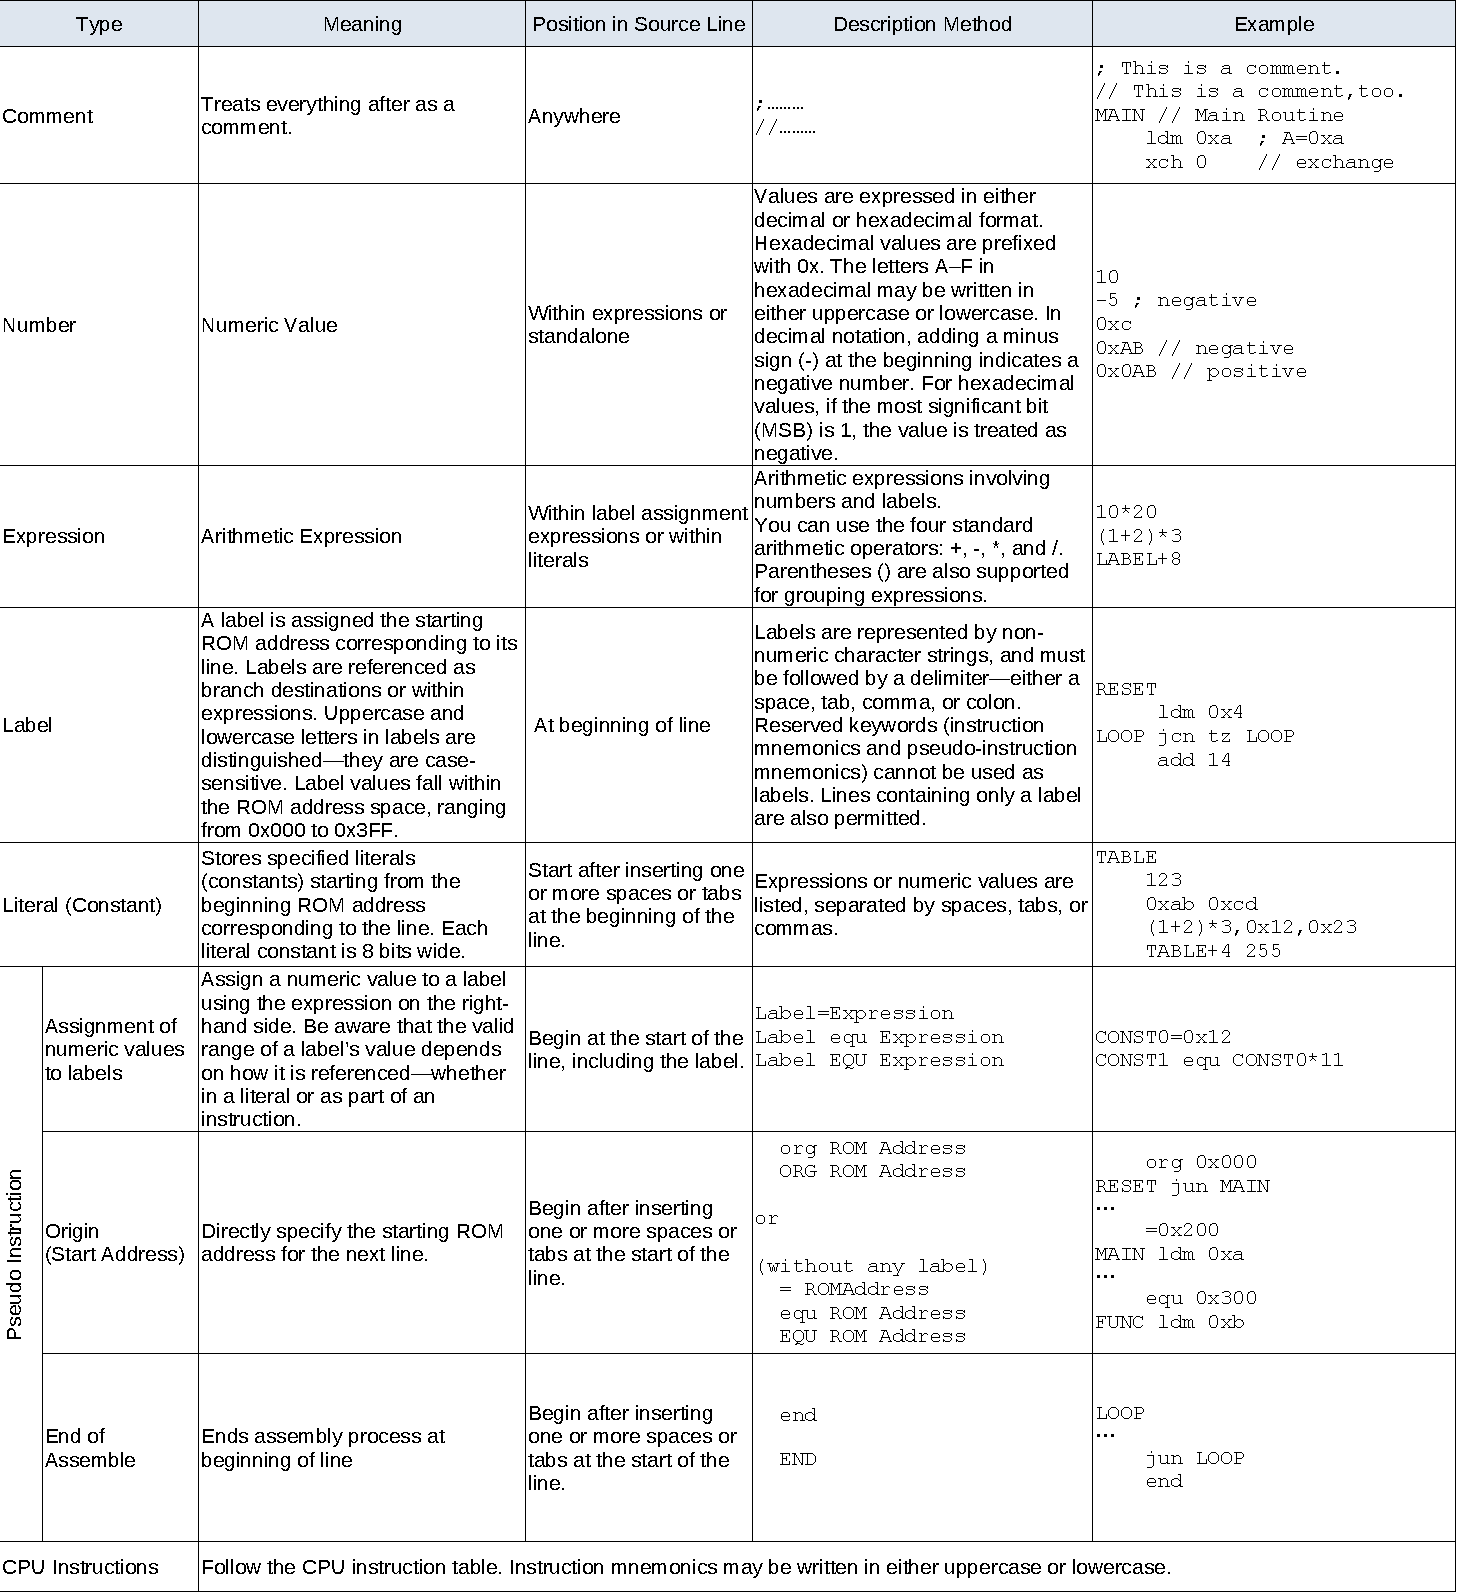
\includegraphics[width=1.00\columnwidth]{./Table/ADS4004AssemblerSyntax.pdf}
    \caption{ADS4004 Assembler Syntax}
    \textit{The assembler syntax used is an original design by the author for the 4004.}
    \label{tb:ADS4004SYNTAX}
\end{table}
%----------------------------------

%==============================================================
\section{ADS4004 Disassembler Functionality}
This section describes how to use the disassembler functionality of ADS4004.  
The input must be a binary file in Intel HEX format.  
Here, we'll disassemble the binary file \texttt{sample.src.hex}, which was generated by assembling the sample program introduced earlier.

To invoke the disassembler, run ADS4004 with the \texttt{-d} option as shown below:\\

\begin{scriptsize}
\begin{boxedverbatim}
$ ./ads4004.exe -d sample.src.hex
\end{boxedverbatim}
\end{scriptsize}
\\

If successful, a disassembled listing file named \texttt{sample.src.hex.lis} will be produced.  
By default, the listing filename is created by appending the extension \texttt{.lis} to the input filename.  
However, you can specify a custom output filename using the \texttt{-l} option.

%==============================================================
\section{ADS4004 CPU Simulator Functionality}
%----------------------------------
\subsection{MCS-4 System Configuration for ADS4004 Simulation}
The CPU simulator feature of ADS4004 is based on the system configuration shown in Table \ref{tb:ADS4004SYSTEMCONFIG}, which assumes an MCS-4 system.  
The ROM/RAM memory capacities are set to their maximum specifications.  
The system includes a feature for self-modification by structuring the ROM described under ``Others'' in Table \ref{tb:ADS4004SYSTEMCONFIG} using RAM; this functionality will be discussed later.

%----------------------------------
\begin{table}
\centering
\begin{tabular}{|l|l|p{9cm}|}
\hline
\rowcolor{LightPurple}
\textbf{Category} & \textbf{Item} & \textbf{Description} \\
\hline
\multirow{5}{*}{ROM} & Number of Chips & 8 units (\#0 to \#7) \\
\cline{2-3}
 & Total Capacity & 4096 bytes (0x000 to 0xFFF) \\
\cline{2-3}
 & Input Port & 4 bits per chip (independent from output port) \\
\cline{2-3}
 & Output Port & 4 bits per chip (independent from input port) \\
\cline{2-3}
 & Number of Banks & 8 banks (\#0 to \#7) \\
\hline
\multirow{4}{*}{RAM} & Chips per Bank & 4 chips per bank, total of 32 units \\
\cline{2-3}
 & Total Capacity & 2560 nibbles = 1280 bytes \\
\cline{2-3}
 & Input Port & 4 bits per chip \\
\cline{2-3}
 & Output Port & 4 bits per chip \\
\hline
Others & \multicolumn{2}{p{11cm}|}{Support for self-modification (WPM instruction) when part of the program memory (typically built with 4001 ROM) is implemented using RAM} \\
\hline
\end{tabular}
\caption{MCS-4 System Configuration for ADS4004 Simulation}
\label{tb:ADS4004SYSTEMCONFIG}
\end{table}
%----------------------------------

%----------------------------------
\subsection{How to use the CPU simulator in ADS4004}
This section explains how to use the CPU simulator in ADS4004.  
The input must be a binary file in Intel HEX format.  
Note that the earlier sample program \texttt{sample.src} was intended only to demonstrate assembler syntax and does not function as a valid program.

For this simulation, we will use the program \texttt{test.src}, which was created to validate the full functionality of ADS4004.

First, assemble the program:\\

\begin{scriptsize}
\begin{boxedverbatim}
$ ./ads4004.exe -a test.src
\end{boxedverbatim}
\end{scriptsize}
\\

Next, launch the ADS4004 simulator using the \texttt{-s} option:\\

\begin{scriptsize}
\begin{boxedverbatim}
$ ./ads4004.exe -s test.src.hex
\end{boxedverbatim}
\end{scriptsize}
\\

The simulation results are output to the log file \texttt{test.src.hex.sim}, which can be reviewed and analyzed later.  
By default, the log filename is generated by appending the extension \texttt{.sim} to the input filename.  
However, you can specify a custom log filename using the \texttt{--log} option.

Upon launching the simulator, the following output will appear.  
All values are displayed in hexadecimal:\\

\begin{scriptsize}
\begin{boxedverbatim}
PC=000 ACC=0 CY=0 R0-15=0000000000000000 DCL=0 SRC=00  (000 40 70    JUN 0x070)
### Q/R/G adr/S/M bnk/P >
\end{boxedverbatim}
\end{scriptsize}
\\

The line beginning with \texttt{PC=...} displays the internal state of the CPU resources—ACC, CY, R0–R15, DCL, SRC—immediately before executing the instruction at address 0x000.  
The instruction code and its disassembled result are shown in parentheses at the far right.


%----------------------------------
\subsection{Interractive Commands of CPU simulator in ADS4004}
When the display begins with \texttt{\#\#\#...}, the simulator is waiting for interactive command input.  
The available interactive commands are shown in Table \ref{tb:ADS4004SIMULATORCOMMAND}.

These commands include:
\begin{itemize}
  \item CPU reset
  \item Execution of instructions until a specified address
  \item Single-step instruction execution
  \item Display of RAM contents
  \item Display of ROM/RAM I/O port states
\end{itemize}

If instruction execution results in abnormal behavior or if you wish to interrupt execution midway,  
press \texttt{Ctrl-C} to return to the interactive command input prompt.

%----------------------------------
\begin{table}
\centering
\begin{tabular}{|p{2.5cm}|p{5cm}|p{6cm}|}
\hline
\rowcolor{LightPurple}
\textbf{Command (case-insensitive)} & \textbf{Function} & \textbf{Remarks} \\
\hline
\texttt{Q} & Exit the simulation & -- \\
\hline
\texttt{R} & Reset the CPU and stop execution & -- \\
\hline
\texttt{G adr} & Run until the Program Counter (PC) reaches address \texttt{adr} & Press \texttt{Ctrl-C} to interrupt.  
Address range (adr): \texttt{000}–\texttt{FFF} (no \texttt{0x} prefix used). \\
\hline
\texttt{S} & Execute one instruction step & -- \\
\hline
\texttt{M bnk} & Display data in RAM bank \texttt{bnk} & Bank number (bnk): \texttt{0}–\texttt{7} \\
\hline
\texttt{P} & Show the state of ROM/RAM I/O ports & -- \\
\hline
\end{tabular}
\caption{ADS4004 Simulator Command List}
\label{tb:ADS4004SIMULATORCOMMAND}
\end{table}
%----------------------------------

The program \texttt{test.src} ultimately halts at an infinite loop instruction \texttt{JUN FINISH} located at address \texttt{0x192}.  
To simulate up to this address, enter the command \texttt{g 192}:\\

\begin{scriptsize}
\begin{boxedverbatim}
### Q/R/G adr/S/M bnk/P >g 192
  PC=070 ACC=0 CY=0 R0-15=0000000000000000 DCL=0 SRC=00  (070 00       NOP)
  PC=071 ACC=0 CY=0 R0-15=0000000000000000 DCL=0 SRC=00  (071 68       INC 8)
...
  PC=0FD ACC=F CY=1 R0-15=A20640EEAB00A040 DCL=0 SRC=00  (0FD D0       LDM 0x0)
  PC=0FE ACC=0 CY=1 R0-15=A20640EEAB00A040 DCL=0 SRC=00  (0FE 11 01    JCN TZ 0x01)
>>>Input TEST Pin Level in Hex (Now 0, RET to unchanged)=
\end{boxedverbatim}
\end{scriptsize}
\\

At this point, the message \texttt{>>>Input TEST Pin Level...} appears and execution halts.  
This occurs before executing the conditional branch instruction \texttt{JCN TZ 0x01}, which depends on the level of the TEST pin.  
To continue simulation, you must specify the input level of the TEST pin (either \texttt{0} or \texttt{1}).  
If the same value as the previous input is desired (initial value is \texttt{0}), simply press Enter.

After repeating this process several times, the following prompt appears:\\

\begin{scriptsize}
\begin{boxedverbatim}
...
  PC=15C ACC=0 CY=1 R0-15=A23440EEAA00A040 DCL=2 SRC=60  (15C 25       SRC 2P)
  PC=15D ACC=0 CY=1 R0-15=A23440EEAA00A040 DCL=2 SRC=40  (15D EA       RDR)
>>>Input ROM(4) Port Level in Hex (Now 0, RET to unchanged)=
\end{boxedverbatim}
\end{scriptsize}
\\

Execution stops again before reaching address \texttt{0x192}.  
This time, the simulator halts prior to executing the \texttt{RDR} instruction, which reads the input level of ROM chip \#4.  
To proceed, enter the 4-bit hexadecimal input level (\texttt{0}–\texttt{F}) for the ROM input port.  
Pressing Enter without input will reuse the previous value (default is \texttt{0}).

Repeat this interaction as needed.  
Once execution reaches the target address, the simulator returns to the interactive command prompt.  
To re-run the simulation from the beginning, use the reset command \texttt{R}.  
To exit, use the quit command \texttt{Q}.

\textbf{Note:} While awaiting input for the TEST pin or ROM input port, interactive commands listed in Table \ref{tb:ADS4004SIMULATORCOMMAND} are \textit{not accepted}.

%==============================================================
\section{4004 CPU Sample Program (1): Memory Access Program – \texttt{memtst.src}}
%----------------------------------
\subsection{Memory Access Program \texttt{memtst.src}}
As a sample program, the memory access program \texttt{memtst.src} is shown in Listing \ref{list:ADS4001MEMTXTSRC}.  
It demonstrates reading and writing operations to the main memory characters of RAM, the status characters of RAM, reading from ROM input ports, writing to ROM output ports, and writing to RAM output ports.  
These instruction sequences are useful as reference patterns for handling such tasks.

Furthermore, the program includes examples using the special instruction \texttt{WPM}, designed for reading and writing to program memory constructed from RAM devices.  
The details of the \texttt{WPM} instruction are explained below.

%----------------------------------
\begin{lstlisting}[caption=Memory Access Program – \texttt{memtst.src}, label=list:ADS4001MEMTXTSRC, captionpos=b,  language=, frame=single, basicstyle=\ttfamily\scriptsize]
// Memory Access Test for ADS4004
        org 0x000 //
MEMTST
        ; RAM W&R
        ldm 1
        dcl
        fim 1P 0x34
        src 1P
        ldm 0xa
        wrm
        ldm 0x5
        rdm

        ; RAM Status Character(RSC) W&R
        ldm 2
        dcl
        fim 2P 0x60
        src 2P
        ldm 0xb
        wr2
        ldm 0x4
        rd2
        rd0

        ; Read ROM Port
        fim 2P 0x40
        src 2p
        rdr

        ; Write ROM Port
        fim 2P 0xc0
        src 2p
        ldm 10
        wrr

        ; Write RAM Port
        ldm 3 ; bank4
        dcl
        fim 3p 0x55
        src 3p
        wmp

        ; ADD RAM
        ldm 2
        dcl
        fim 1P 0x56
        src 1P
        ldm 0xa
        wrm
        stc ; Carry=1
        ldm 0x6
        adm

        ; SUB RAM
        ldm 2
        dcl
        fim 1P 0x57
        src 1P
        ldm 0x5
        wrm
        stc ; Borrow=0
        ldm 0x6
        sbm

        ; Program RAM R&W
        ldm 0
        dcl
        fim 0p 0
        src 0p
        ldm 0x0
        wr0
        ldm 0x2
        wr1
        ldm 0x4
        wr2
        ;
        jms PGM_RD
        ;
        fim 1P 0xab
        jms PGM_WR
        ;
        fim 1P 0x0
        jms PGM_RD

// End of Test
FINISH jun FINISH

// Program RAM, Read & Write
//   Program RAM Location = Bank0, Chip0, Reg0: {RSC0, RSC1, RSC2}
//   Program RAM Data = {R2:R3}
PGM_WR
        fim 0p 224
        src 0p
        ldm 1
        wrr
        jms PGMCOM
        ld  2
        wpm
        ld  3
        wpm
        fim 0p 224
        src 0p
        clb
        wrr
        bbl 0
PGM_RD
        jms PGMCOM
        wpm
        wpm
        fim 0p 224
        src 0p
        rdr
        xch 2
        inc 0
        src 0p
        rdr
        xch 3
        bbl 0
PGMCOM
        fim 0p 0
        src 0p
        rd1
        xch 10
        rd2
        xch 11
        rd0
        fim 0p 240
        src 0p
        wrr
        src 5p
        bbl 0

        end  ; end of assemble source
\end{lstlisting}
%----------------------------------

%----------------------------------
\subsection{Special Instruction \texttt{WPM} for Program RAM Access}
The \texttt{WPM} instruction is used to access ``program RAM''—a portion of program memory typically built from 4001 ROM, but here implemented using RAM devices.  
Although the execution timing of \texttt{WPM} follows that of WR-type instructions (as shown in Figure \ref{fig:CPUINSTRUCTIONREAD}), it is used not only for writing but also for reading program RAM.

%----------------------------------
\subsection{External Hardware Support Required for \texttt{WPM}}
Accessing program RAM via \texttt{WPM} requires external hardware support.  
This hardware monitors CPU fetch cycles for \texttt{WPM} and performs the necessary operations.  
It uses the I/O ports of ROM chips \#14 and \#15 for reading and writing to program RAM.  
Since both input and output ports are used simultaneously, the standard 4001 cannot handle this.  
Instead, the support hardware must emulate the port functionality of chips \#14 and \#15.

The ADS4004 simulator emulates this integrated behavior, including the interaction between the \texttt{WPM} instruction and support hardware.  
Additionally, it allows for reading and writing the ROM content of 4001 chips—functionality not available in actual hardware.

%----------------------------------
\subsection{Operation When Writing to Program RAM via \texttt{WPM}}
The following sequence is performed when writing to program RAM:

\begin{enumerate}
  \item Write the value \texttt{0x1} to the output port of ROM chip \#14 to signal the start of a program RAM write.
  \item Write the upper 4 bits of the 12-bit program RAM address to the output port of ROM chip \#15.
  \item Output the lower 8 bits of the address via the \texttt{SRC} instruction to the data bus.
  \item Perform two executions of the \texttt{WPM} instruction:
    \begin{itemize}
      \item First \texttt{WPM} writes the upper 4 bits from the accumulator (ACC).
      \item Second \texttt{WPM} writes the lower 4 bits from ACC.
    \end{itemize}
    The hardware counts the executions to determine which half is being written.
  \item Write the value \texttt{0x0} to the ROM chip \#14 output port to signal the end of write operation.
\end{enumerate}

%----------------------------------
\subsection{Operation When Reading from Program RAM via \texttt{WPM}}
Reading from program RAM via \texttt{WPM} follows this sequence:

\begin{enumerate}
  \item Write the upper 4 bits of the 12-bit program RAM address to the output port of ROM chip \#15.
  \item Output the lower 8 bits of the address via the \texttt{SRC} instruction.
  \item Perform two executions of the \texttt{WPM} instruction:
    \begin{itemize}
      \item First \texttt{WPM} causes the upper 4 bits of data to appear at ROM chip \#14's input port.
      \item Second \texttt{WPM} causes the lower 4 bits to appear at ROM chip \#15's input port.
    \end{itemize}
    These values are then acquired using the \texttt{RDR} instruction.  
    The support hardware handles the bit selection based on execution count.
\end{enumerate}

%----------------------------------
\subsection{Accessing Program RAM in Sample Program \texttt{memtst.src}}
In Listing \ref{list:ADS4001MEMTXTSRC}, the sample program writes to program RAM by encoding the 12-bit target address into RAM bank \#0, chip \#0, register \#0 status characters:
\begin{itemize}
  \item Upper 4 bits → status character~0
  \item Middle 4 bits → status character~1
  \item Lower 4 bits → status character~2
\end{itemize}
The write data (8 bits) is stored in index register pair R1P (R2, R3) before calling the subroutine \texttt{PGM\_WR}.

To read from program RAM, the same address encoding is performed, followed by calling \texttt{PGM\_RD}, which places the read data into R1P.

%----------------------------------
\subsection{Simulation of Sample Program \texttt{memtst.src}}
Let's simulate \texttt{memtst.src} using ADS4004:\\

\begin{scriptsize}
\begin{boxedverbatim}
$ ./ads4004.exe -a memtst.src
$ ./ads4004.exe -s memtst.src.hex
\end{boxedverbatim}
\end{scriptsize}
\\

The program ends at address \texttt{0x4B}, so execute until then:\\

\begin{scriptsize}
\begin{boxedverbatim}
### Q/R/G adr/S/M bnk/P >g 4b
\end{boxedverbatim}
\end{scriptsize}
\\

During execution, the program will request input for ROM chip \#4’s input port during an \texttt{RDR} instruction.  
You can press Enter to accept the default value.\\

\begin{scriptsize}
\begin{boxedverbatim}
>>>Input ROM(4) Port Level in Hex (Now 0, RET if unchanged)=
\end{boxedverbatim}
\end{scriptsize}
\\

In the subroutine \texttt{PGM\_RD}, inputs to ROM chips \#14 and \#15 are requested prior to \texttt{RDR} execution.  
The simulator automatically provides the correct program memory value to the corresponding input port, so pressing Enter is sufficient:\\

\begin{scriptsize}
\begin{boxedverbatim}
>>>Input ROM(14) Port Level in Hex (Now 2, RET if unchanged)=
...
>>>Input ROM(15) Port Level in Hex (Now 2, RET if unchanged)=
...
>>>Input ROM(14) Port Level in Hex (Now a, RET if unchanged)=
...
>>>Input ROM(15) Port Level in Hex (Now b, RET if unchanged)=
\end{boxedverbatim}
\end{scriptsize}

%==============================================================
\section{4004 CPU Sample Program (2): BCD to Binary Conversion – \texttt{bcd2bin.src}}
%----------------------------------
\subsection{BCD to Binary Conversion – \texttt{bcd2bin.src}}
This sample program, \texttt{bcd2bin.src}, performs conversion from BCD code (Binary Coded Decimal) to binary (BIN). The source program is shown in Listing \ref{list:ADS4001BCD2BINSRC}.
The supported BCD range is from 0 to 255.  
For example, BCD value \texttt{123} is converted to binary \texttt{0x7B}.

%----------------------------------
\begin{lstlisting}[caption=BCD to Binary Conversion – \texttt{bcd2bin.src}, label=list:ADS4001BCD2BINSRC, captionpos=b,  language=, frame=single, basicstyle=\ttfamily\scriptsize]
// BCD to BIN for ADS4004
    org 0x000

    // Main Routine
MAIN
    // Store BCD in Bank0/Chip0/Reg0/Chr2-Chr0
    ldm 0
    dcl
    fim 0p 0x02
    src 0p
    ldm 0x1   ; MSB of BCD Code
    wrm
    fim 0p 0x01
    src 0p
    ldm 0x2   ; Middle of BCD Code
    wrm
    fim 0p 0x00
    src 0p
    ldm 0x3   ; LSB of BCD Code
    wrm
    // Call BCD to BIN Converter
    jms BCDBIN
    // Store BIN Result in Bank0/Chip0/Reg0/Chr4-Chr3
    fim 0p 0x04
    src 0p
    xch 2     ; MSB of R1P (Result)
    wrm
    fim 0p 0x03
    src 0p
    xch 3     ; LSB of R1P (Result)
    wrm
FINISH
    jun FINISH    
    
// Convert BCD to Binary
BCDBIN
    fim 0p 0   ; R0P=0
BCDBIN_1 // 1st Digit
    fim 1p 0   ; R1P=0 (Result)
    src 0p
    rdm        ; Read 1st (LSB) BCD Digit
    xch 3      ; R1P(LSB)=1st BCD Digit
BCDBIN_2 // 2nd Digit
    fim 2p 10  ; R2P=10, for 2nd Digit
    jms BCDADD ; Repeat (R1P=R1P+R2P) for Digit times
BCDBIN_3 // 3rd Digit
    fim 2p 100 ; R2P=100, for 3rd Digit
    jms BCDADD ; Repeat (R1P=R1P+R2P) for Digit times
BCDBIN_END
     bbl 0     ; Return
BCDADD
    inc 1      ; R1=R1+1
    src 0p     ; Prepare to Read Next Digit
BA1
    rdm        ; Read the BCD Digit
    jcn az BA2 ; if ACC==0, jump to BA2
    dac        ; ACC=ACC-1
    wrm        ; Write Back the Decremented BCD Digit to RAM
    clc        ; R1P=R1P+R2P
    ld 3       ;   ACC=R3
    add 5      ;   ACC=ACC+R5
    xch 3      ;   R3=ACC
    ld 2       ;   ACC=R2
    ADD 4      ;   ACC=ACC+R4
    xch 2      ;   R2=ACC
    jun BA1    ; jump to BA1
BA2
    bbl 0      ; Return

    end
\end{lstlisting}
%----------------------------------

%----------------------------------
\subsection{Conversion Algorithm}
The conversion algorithm is simple.  
Take the BCD code \texttt{123} as an example.  
The binary result is calculated as follows:
\begin{itemize}
  \item Store the lowest BCD digit (\texttt{3}) in the binary result.
  \item Add \texttt{10} to the result for each count of the middle BCD digit (\texttt{2} times).
  \item Add \texttt{100} to the result for each count of the highest BCD digit (\texttt{1} time).
\end{itemize}

%----------------------------------
\subsection{Program Description}
The core subroutine for conversion is named \texttt{BCDBIN}.  
The input BCD code is stored in RAM bank \#0 at SRC addresses \texttt{0x00}–\texttt{0x02} (from least to most significant digit).  
After calling \texttt{BCDBIN}, the converted binary value is stored at addresses \texttt{0x03}–\texttt{0x04}, also in bank \#0, with the lower byte first.

%----------------------------------
\subsection{Simulation Using ADS4004}
To simulate the sample program using ADS4004:\\

\begin{scriptsize}
\begin{boxedverbatim}
$ ./ads4004.exe -a bcd2bin.src
$ ./ads4004.exe -s bcd2bin.src.hex
\end{boxedverbatim}
\end{scriptsize}
\\

Run the program up to address \texttt{0x11}, where the BCD input is set and \texttt{BCDBIN} is called:\\

\begin{scriptsize}
\begin{boxedverbatim}
### Q/R/G adr/S/M bnk/P >g 11
  PC=001 ACC=0 CY=0 R0-15=0000000000000000 DCL=0 SRC=00  (001 FD       DCL)
  PC=002 ACC=0 CY=0 R0-15=0000000000000000 DCL=0 SRC=00  (002 20 02    FIM 0 0x02)
...
  PC=010 ACC=3 CY=0 R0-15=0000000000000000 DCL=0 SRC=00  (010 E0       WRM)
  PC=011 ACC=3 CY=0 R0-15=0000000000000000 DCL=0 SRC=00  (011 50 1F    JMS 0x01F)
### Q/R/G adr/S/M bnk/P >m 0
Bank=0 Chip=0 Reg=0 Addr=000  3 2 1 0 0 0 0 0 0 0 0 0 0 0 0 0  Status= 0 0 0 0
Bank=0 Chip=0 Reg=1 Addr=010  0 0 0 0 0 0 0 0 0 0 0 0 0 0 0 0  Status= 0 0 0 0
Bank=0 Chip=0 Reg=2 Addr=020  0 0 0 0 0 0 0 0 0 0 0 0 0 0 0 0  Status= 0 0 0 0
...
\end{boxedverbatim}
\end{scriptsize}
\\

Now continue execution up to address \texttt{0x1D} and verify that the binary result \texttt{0x7B} is stored correctly:\\

\begin{scriptsize}
\begin{boxedverbatim}
### Q/R/G adr/S/M bnk/P >g 1d
  PC=01F ACC=3 CY=0 R0-15=0000000000000000 DCL=0 SRC=00  (01F 20 00    FIM 0 0x00)
  PC=021 ACC=3 CY=0 R0-15=0000000000000000 DCL=0 SRC=00  (021 22 00    FIM 2 0x00)
...
  PC=01B ACC=7 CY=0 R0-15=030B640000000000 DCL=0 SRC=03  (01B B3       XCH 3)
  PC=01C ACC=B CY=0 R0-15=0307640000000000 DCL=0 SRC=03  (01C E0       WRM)
### Q/R/G adr/S/M bnk/P >m 0
Bank=0 Chip=0 Reg=0 Addr=000  3 0 0 b 7 0 0 0 0 0 0 0 0 0 0 0  Status= 0 0 0 0
Bank=0 Chip=0 Reg=1 Addr=010  0 0 0 0 0 0 0 0 0 0 0 0 0 0 0 0  Status= 0 0 0 0
Bank=0 Chip=0 Reg=2 Addr=020  0 0 0 0 0 0 0 0 0 0 0 0 0 0 0 0  Status= 0 0 0 0
\end{boxedverbatim}
\end{scriptsize}
\\

Follow the progression of CPU resources and memory state to deepen your understanding of the 4004 CPU operation and verify correctness of your implementation.
%==============================================================
